% Robin

\begin{frame}
\frametitle{Neural Networks}
\begin{itemize}
\item Neural networks are a type of machine-learning model inspired by the structure of the human brain.
\begin{figure}[h]
\centering
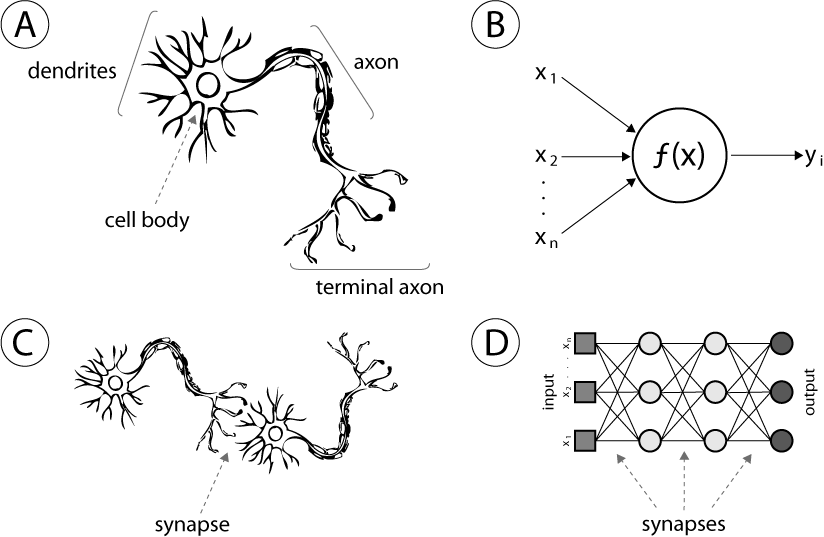
\includegraphics[width=0.7\textwidth]{figures/neural_brain.png}
% \caption{My image with a reference \cite{https://wp.nyu.edu/yungjurick/2020/03/15/debate-on-the-relationship-between-neural-network-and-the-brain/}}
% \label{fig:my_image}
\end{figure}
\item Neural networks can learn to recognize patterns and make predictions based on input data, and can be used for image and speech recognition, natural language processing, etc.

\end{itemize}
\end{frame}

% \begin{frame}
% \frametitle{Neural Networks}
%     % \begin{neuralnetwork}[height=4]
%     %     \newcommand{\x}[2]{$x_#2$}
%     %     \newcommand{\y}[2]{$\hat{y}_#2$}
%     %     \newcommand{\hfirst}[2]{\small $h^{(1)}_#2$}
%     %     \newcommand{\hsecond}[2]{\small $h^{(2)}_#2$}
%     %     \inputlayer[count=3, bias=true, title=Input\\layer, text=\x]
%     %     \hiddenlayer[count=4, bias=false, title=Hidden\\layer 1, text=\hfirst] \linklayers
%     %     \hiddenlayer[count=3, bias=false, title=Hidden\\layer 2, text=\hsecond] \linklayers
%     %     \outputlayer[count=2, title=Output\\layer, text=\y] \linklayers
%     % \end{neuralnetwork}
% \begin{itemize}
% \end{itemize}
% \end{frame}

\begin{frame}
\frametitle{Generative Adversarial Network (GAN)}
\begin{itemize}
\item GAN is a specific type of neural network that are used for generating new data that is similar to a given dataset.
\item GAN consists of two neural networks: a generator and a discriminator.
\begin{figure}[h]
\centering
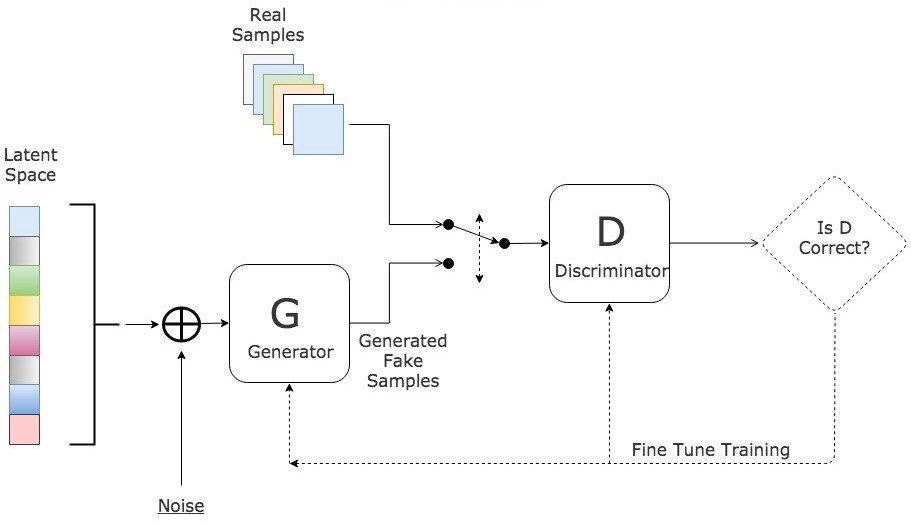
\includegraphics[width=0.8\textwidth]{figures/gan.jpeg}
% \caption{My image with a reference \cite{https://wp.nyu.edu/yungjurick/2020/03/15/debate-on-the-relationship-between-neural-network-and-the-brain/}}
% \label{fig:my_image}
\end{figure}
\end{itemize}
\end{frame}
